\section{Experiment and Discussion}
\subsection{Evaluation for Co-segmentation on Synthetic Data}
\begin{figure}[htb]
	\centering
	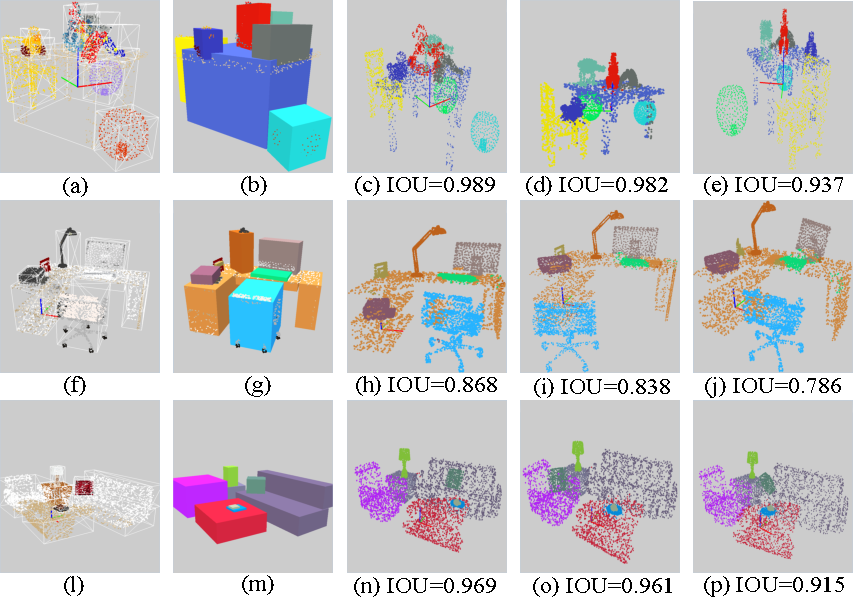
\includegraphics[width=\linewidth]{images/seg/seg}
	\caption{\label{fig:seg}Three rows in the figure shows segmentation evaluations on three groups of synthetic data(child table, office desk, living room). Each group of data have 13 point sets. The first column are examples of point sets for each group of data. The second column are mannual placed layout for each group of data. The $3^{rd}$ column shows the segmentation result with maximum IOU scores in the groups. The $4^{th}$ column shows the segmentation result with median IOU scores in the groups. The $5^{th}$ column shows the segmentation result with minimum IOU scores in the groups.}
\end{figure}
From the perspective of co-segmentation, we evaluate our algorithm on synthetic data of indoor scenes. To estimate the power of the algorithm we only input layout for one point set in each group for initialization and do not use the hot intervention mechanism. For this evaluation, we think that the color feature is too strong an indication for segmentation in the synthetic data (there is no shadow and lighting variation that will bring in more challenges for segmentation). Using color feature with the bilateral formulation prevents us from doing a fair evaluation of our algorithm, but we need the ground truth of segmentation comes with synthetic data to do the evaluation. For the above reasons, we use only basic formulation for the evaluation of co-segmentation, and no color information is used for optimization. For the estimation, we calculate the intersection over union (IOU) scores for the result segmentation against ground-truth segmentation. We generate three group of synthetic point sets and each group have 13 point sets as inputs. The Figure~\ref{fig:seg} shows the result of the evalution.\\
From the evaluation, we want to discuss two observations:\\
Firstly, for all three groups, the point set with highest IOU score is not the same as the point set equiped with mannually placed layout.In other words , the point sets from the $3^{rd}$ column in Figure~\ref{fig:seg} are not the same point sets from $2^{nd}$. We believe this is because that the mannually placed layout is not accurate respecting to point-wise segmentation. At early iterations of the optimization, the alteration in (\ref{equ:alteralpha}) can serve as a soft constraint to help constratining the shape of object, but in the final iterations the alteration will obstruct the further improvement of segmentation for the correspondent point set. 
\subsection{Evaluation for Joint Registration on Synthetic Data}
In the process of generating synthetic data, we didn't record the groundtruth of the transformation of the 
\subsection{Test On Real Data}
\begin{figure*}[htb]
	\centering
	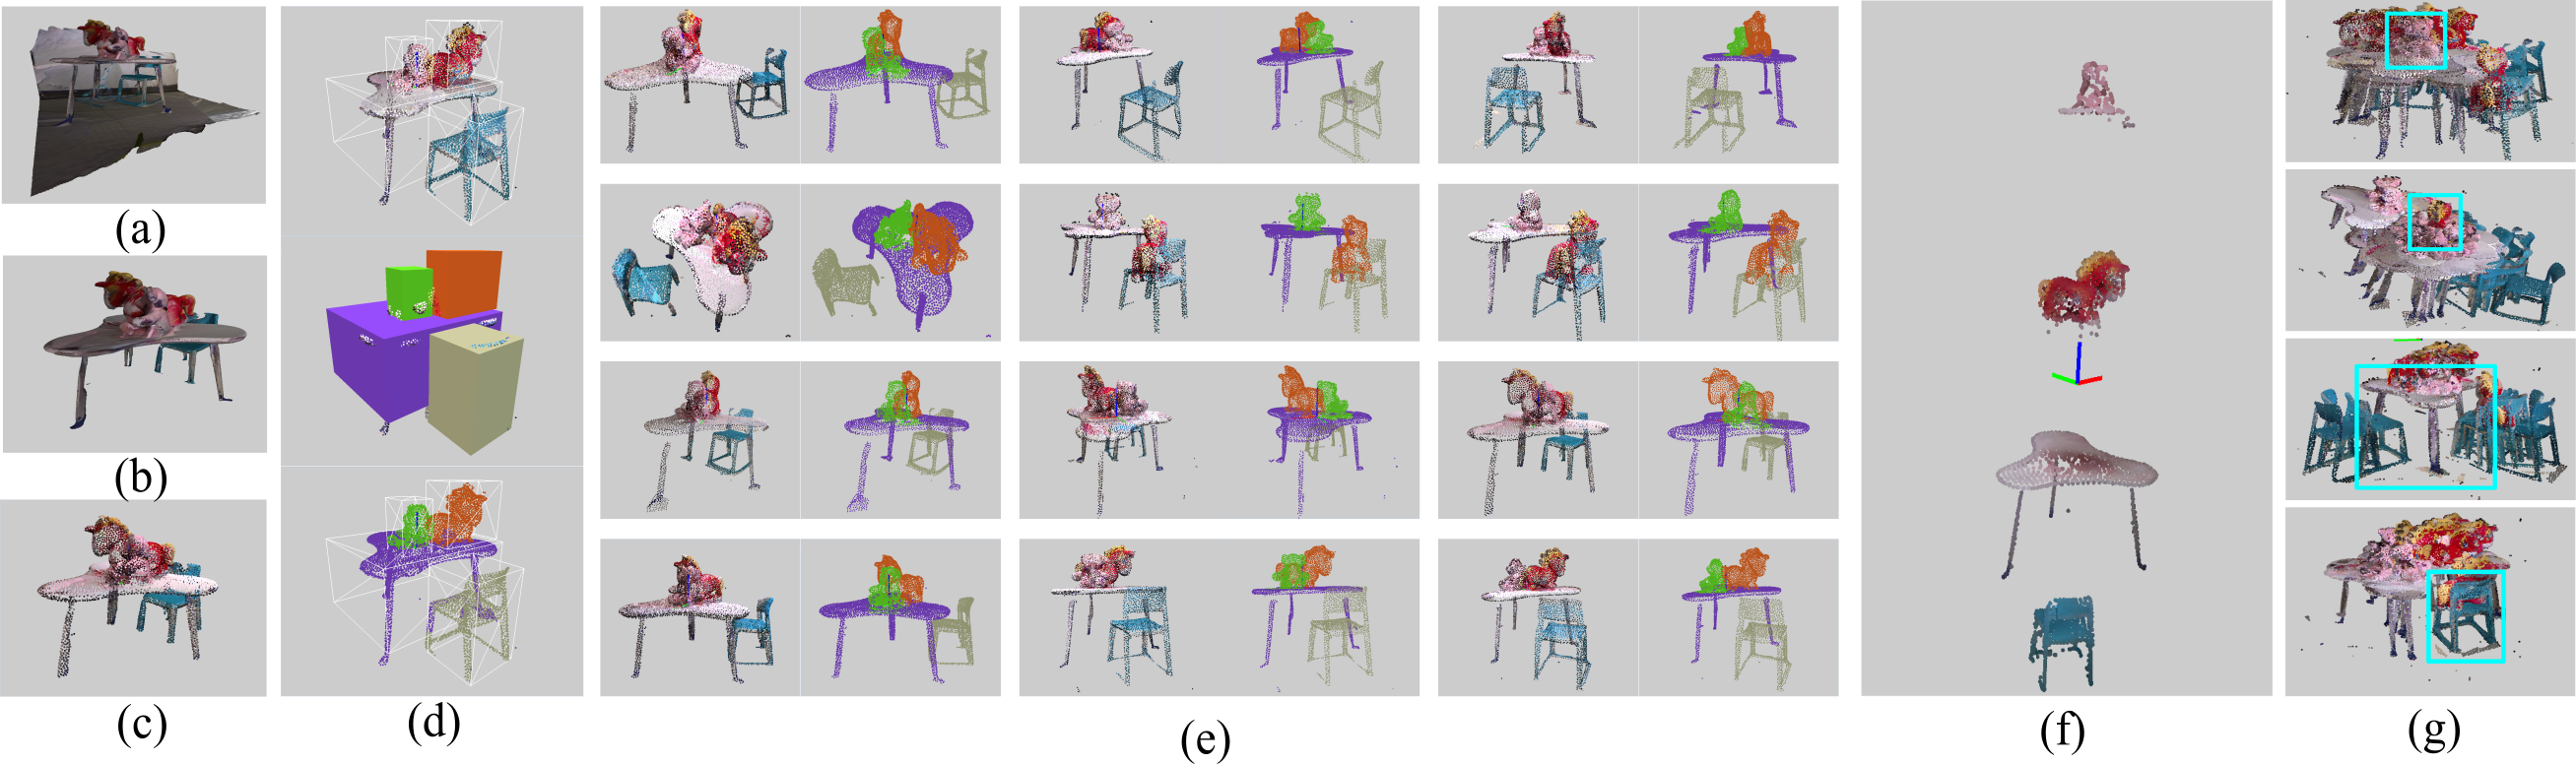
\includegraphics[width=\linewidth]{images/realdata/realdata}
	\caption{\label{fig:realdata}This figure shows our test on a real data. (a)(b)(c) shows how we capture real data and convert to input point set. (d) shows the first input point set, the input layout on it and its segmentation result. (e) shows pairs of other input point sets and corresponding segmentation result. (f) shows the final Gaussian centroids. (g) verifys the registration result by aligning input point sets respecting to each object. The light blue rectangle highlights the object that is aligned together. }
\end{figure*}
We test our algorithm on a set of real data, Figure~{\ref{fig:realdata}} shows the result of our test.
\subsection{Limitations and Future Work}
